%%%%%%%%%%%%%%%%%%%%%%%%%%%%%%%%%%%%%%%%%
% University/School Laboratory Report
% LaTeX Template
% Version 3.1 (25/3/14)
%
% This template has been downloaded from:
% http://www.LaTeXTemplates.com
%
% Original author:
% Linux and Unix Users Group at Virginia Tech Wiki 
% (https://vtluug.org/wiki/Example_LaTeX_chem_lab_report)
%
% License:
% CC BY-NC-SA 3.0 (http://creativecommons.org/licenses/by-nc-sa/3.0/)
%
%%%%%%%%%%%%%%%%%%%%%%%%%%%%%%%%%%%%%%%%%

%----------------------------------------------------------------------------------------
%	PACKAGES AND DOCUMENT CONFIGURATIONS
%----------------------------------------------------------------------------------------

\documentclass{article}

\usepackage[utf8]{inputenc}
\usepackage{graphicx} % Required for the inclusion of images
%\usepackage{natbib} % Required to change bibliography style to APA
\usepackage{amsmath} % Required for some math elements 
\usepackage{glossaries}
\usepackage[toc,page]{appendix}
\usepackage[autostyle=true]{csquotes}
\usepackage{hyperref}

\setlength\parindent{0pt} % Removes all indentation from paragraphs

%\usepackage{times} % Uncomment to use the Times New Roman font

%----------------------------------------------------------------------------------------
%	DOCUMENT INFORMATION
%----------------------------------------------------------------------------------------

\title{Reserach-proposal} % Title

\author{Jonathan \textsc{Thaler}} % Author name

\date{\today} % Date for the report

\begin{document}

\maketitle % Insert the title, author and date

% If you wish to include an abstract, uncomment the lines below
\begin{abstract}
This paper describes the idea, aim and impact of the PhD study do be undertaken.
\end{abstract}


\section{Introduction}
There exists a large number of simulation packages which allow the convenient creation of System Dynamics simulations by straight-forward visual diagram creation. One simply creates stocks and flows, connects them, specifies the flow-rates and initial parameters and then runs the model. An example for such a visual diagram creation in the simulation package AnyLogic can be seen in Figure \ref{fig:sir_stockflow_diagram}.

\begin{figure}
	\centering
	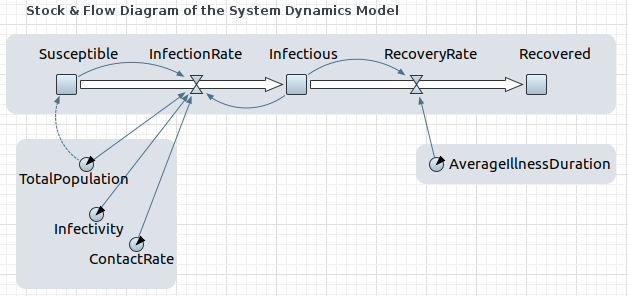
\includegraphics[width=.5\textwidth, angle=0]{./fig/SIR_SD_STOCKFLOW_DIAGRAMM.png}
	\caption{Visual System Dynamics Diagram of the SIR model in AnyLogic Personal Learning Edition 8.3.1.}
	\label{fig:sir_stockflow_diagram}
\end{figure}

Still, implementing System Dynamics directly in code is not as straight forward and involves numerical integration which can be quite tricky to get right. Thus, the aim of this paper is to look into how System Dynamics models can be implemented in code correctly without the use of a simulation package. We use the well known SIR model \cite{kermack_contribution_1927} from epidemiology to demonstrate our approach.

Our language of choice is Haskell because it emphasises a declarative programming style in which one describes \textit{what} instead of \textit{how} to compute. Further it allows to rule out interference with non-deterministic influences or side-effects already at compile-time. This is of fundamental importance for System Dynamics because it behaves completely deterministic and involves no stochastics or non-determinism whatsoever. Also, we make use of Functional Reactive Programming which allows to express continuous-time systems in a functional way. 

We show that by this approach we can arrive at correct-by-construction implementations of System Dynamic models. This means that the correctness of the code is obvious because we have closed the gap between the model specification and its implementation. Thus, the contribution of the paper is the demonstration of how to implement correct-by-construction System Dynamics simulations using Haskell and Functional Reactive Programming.

\section{Project-Plan}

\subsection{Years}
The whole PhD lasts for 3 years and thus I will structure it according to 3 years where each year will be a major milestone - which is also intended by the Computer School.

\subsubsection{1st Year: Basics}
In this year I will learn basics and develop and research the methodology I will use for the main work in the 2nd year. Also I want to write a paper of how to apply functional programming to ABM/S. The time-frame will be set by the date of the 1st year annual oral report which will happen beginning of July thus there are about 6 Months time (counting including January '17 and leaving out July '17). These are the things I want / need to achieve this year:

\begin{itemize}
\item Prototyping in Haskell, Scala and Java
\item Study Actor-Model theory: Hewitt, Greif, Clinger, Agha
\item Get into reasoning about programs
\item Basics of Economics \cite{bowles_understanding_2005}, \cite{kirman_complex_2010}
\item Basics of ACE: Tesfatsion
\item Implement PureAgents Library
\item Write the paper
\item Write 
\item Prototype Auction/Fishmarket using Akka and Haskell and describe results in 1st year report.
\item Write 1st year report
\end{itemize}

Important and mile-stone dates:

\begin{center}
\begin{tabular}{ c|c } 
	April (End) & Finished Paper: functional ABM \\ 
	\hline
	June (Mid) & Finished writing 1st year report  \\ 
	\hline
	July & Oral annual report \\
\end{tabular}
\end{center}

TODO-List as of \today

\begin{itemize}
\item send abstract
\item investigate speed of divergence of simulation runs using the terminology of gleichzeitige ungleichzeitigkeiten
\item 2 complex system can lead to a total different outcome when initial settings differ only by fractions. thus it may also be the case for specific ABM/S?
\item todo: render paths of the agents in heroes and cowards
\item todo: abm/s of a go game
\item IDEA: what about an ABM/S of karma and rebirth? add to genesis paper
\item IDEA: what about ABM/S generating sound? could be a perfect example for Yampa due to its signal functions. the sound is the result of interactions of agents which try to generate harmonies and agents trying to create dissonance
\item IDEA: what about abm/s creating drawings/art? 2d continuous and each agents path is drawn
\item haskell: dont have objects with methods which can call between each other but we need some way of representing agents. this is done using a struct type with a behaviour function and messaging mechanisms. important: agents are not carried arround but messages are sent to a receiver identified by an id. 
\item messaging mechanisms have up- and downsides, elaborate on it.
\item reason for patterns: heroes try to stay 50 \% in between and have selected 2 cowards which themselves are at the borders opposite. need much more cowards than heroes 75/25. TODO: investigate pair-wise movement.
\item hypothesis: individual runs diverge from the first step on but the global behaviour stays the same.
\item question: do emergent patterns break down / global dynamics change completely in some ABM/S when changing sim-semantic? which kind of ABM could show this behaviour? which properties are responsible for it?
\item parallel more natural in haskell
\item sequential more natural in java
\item concurrent difficult in both, using stm in haskell it becomes very natural, STM available in java too. actors are an even better approach but is having problems with time in simulation
\item implement conways game of life: parallel discrete: read global environment, write local
\item implement schelling segregation
\item generalize 2d grid-renderer: agentToCell maps agent to color and discrete 2d - coord
\item generalize 2d continuous renderer: color, position and direction
\item implement simtime Actors
\item only one function: agenttransformer. replace update by call to agenttransformer with message "DT" and parameter dt. add mechanism to add sys messages
\item implement sequential version: PureAgentsSeq. should be easy starting from par version. implement environment accesslike STM: each agent can read/write complete env
\item implement environment for parallel
\item performance unacceptable: 1000 in haskell vs 100.000 in java is a shame on haskell, more should be possible
\item implement SIRS on a 8neighbourhood grid (nearly the same as wildfire). difference only in neighbourhood filter, rest of code should be same (sendrandomagent)
\item send abstract to peer and thorsten in 1st week of january. try to submit paper on SIMPAT with deadline of 30th april
\item embed PureAgentsPar in Yampa: PureAgentsYampa
\item implement agent monad: PureAgentsMonadic. but what is an Agent-Monad?
\item when having agent monad, run in dunai
\item look into QuickCheck and HPC
\item problem: so far only agents with same static messagetypes, environment and states, can communicate: the agents are homogenous. how can we implement hetereogenous agents in this library?
\item run PureAgents inside Dunai/Yampa
\item where does 1st and 2nd year research meet: reasoning about emergent properties of the simulation. in case of HAC the crosspattern, in case of ACE the convergence to stable prices

\item Continue investigations regarding the heroes and cowards game
\item Explore the literature on complex systems to find an explanation for the emergence of the macro level patterns in the Heroes \& Cowards game
\item Consider the next step: Implementing an economics example at different levels of complexity 
\item Continue writing conference paper and looking out for an appropriate conference

\item paper abstract: local-only immutable data, explicit dataflow, higher order functions and recursion
\item paper: we also present a novel approach to implementing ABM/S by implementing 3 of the semantics in pure functional Haskell and comparing them to OO Java and examine for which semantics boths methods are well suited an which not.
\item paper: contribution: 1. development of terminology of simulation semantics 2. pure functional approach and comparison to state-of-the-art oo 3. influence of semantics on dynamics 4. reasoning about dynamics
\end{itemize}

\paragraph{January}
TODO

\paragraph{February}
TODO

\paragraph{March}
TODO

\paragraph{April}
TODO

\paragraph{May}
TODO

\paragraph{June}
TODO

\paragraph{July}
TODO


\subsubsection{2nd Year: Main Work}
Applying 1st year results, methods and experiences to develop and write main paper to be published in a journal in 3rd year thus in 2nd year the main  work and implementation will be done. The idea is to start from Ionescus Framework \cite{Botta20114025} and build on his paper.

\begin{itemize}
\item Implement Ionescous framework using the methodology developed in 1st year
\item Generalize implementation to market models
\item Learn Agda and dependent types
\item Dig deeper into equilibrium theory 
\item Get into market-microstructure: \cite{LehalleLaruelle2013}, \cite{baker_market_2013}
\item Dig into \textit{emergent properties} of systems. Can they be formalized?
\item Get into basics of Category-Theory \cite{Pierce1991} \cite{spivak_category_2014}
\item Get into basics of Type-Theory (found good lectures on Youtube)

\end{itemize}

\subsubsection{3rd Year: Finalizing, Publishing \& Writing}
I plan to be finished - or nearly finished - at the end of the 3rd year. In this year I will finalize the work of the 2nd year, publish the my main journal paper (and optional fun-papers if possible) and will write down the thesis. \\ To have a bit of distraction and to prevent myself to become too locked in in writing on the thesis I will also work on my optional fun-papers (see below) and hope to at least finish them and maybe publish them - at least I want to present them to 2-3 audiences (e.g. FP Lunch) to test the reaction (especially the Genesis-Paper).

\begin{itemize}
\item Finalize research of 2nd year
\item Publish journal paper
\item Write thesis
\item Work on fun-papers
\end{itemize}

\subsection{Papers}
This is the list of papers I want to work on. The goals of publishing I set for myself are given beside the paper.

\begin{enumerate}
\item \textit{Dynamics of Agent-Based Simulation \& Modelling under different Simulation-Semantics.} - Conference paper
\item \textit{Pure Functional ACE (Catchy title yet to be defined)} - Journal paper
\item \textit{Pure by Nature: A Library for pure Agent-Based Simulation \& Modelling in Haskell} - Journal paper ?
\item \textit{Time in Games: a Tron Light-Cycle Game in Dunai} - Journal/Conference paper
\item \textit{The Genesis According to Computer-Science: Reality as Simulation of Free Will} - Optional publishing
\item \textit{Pure Functional Islamic Design} - Optional publishing
\end{enumerate}

\subsubsection{Dynamics of Agent-Based Simulation \& Modelling under different Simulation-Semantics.}
The first paper which describes how one can implement ABM/S in Haskell and compares the implementation and results to Java and Akka. A major focus are update-strategies, parallelism, reproducibility, reasoning and comparability between the various implementations. 

Actors: The Future in Agent-Based Simulation \& Modelling?
Although the actor-model is quite old (beginning of the 70s) it seems to have a revival both in Erlang in the 90s and now in the Framework Akka (based on Scala). It is one way of organizing highly parallel (and optionally distributed) applications. Also the actor-model is very close to the agent-metaphor where the latter one was strongly inspired by the former one. Thus It would be very interesting to look closer into how the Actor-Model can be utilized to ABM/S as it seems that this has not been properly done yet.

This paper will establish my methodology in using Haskell / pure functional programming in the 2nd year main work.

\subsubsection{Pure Functional ACE (Catchy title yet to be defined)}
Is the main work of the PhD and targeted at publication in a Journal. The exact topic and content will be clarified at the beginning of the 2nd year. Mainly it will describe how to implement Ionescus Framework of Gintis trading model and extend it to a more general Market-Model. It will also give an outlook on implementing it using dependent types.

\subsubsection{Pure by Nature: A Library for pure Agent-Based Simulation \& Modelling in Haskell}
This paper describes the ideas and theory behind the implementation of my ABM/S library "PureAgents" in Haskell.

\subsubsection{Time in Games: a Tron Light-Cycle Game in Dunai}
This paper describes the 2D light-cycle game inspired by the movie Tron implemented in Dunai. It allows to turn back time.

\subsubsection{The Genesis According to Computer-Science: Reality as Simulation of Free Will}
I've always been interested in a deeper meaning behind things so I want to look into the philosophy and future of simulation: why do we simulate, what can we derive from simulations, what does it say that we humans simulate, what will the future of simulation be? \\
I claim that our ability to "simulate" in our mind separates our intelligence from those of the animals and that this is a unique property of humans. Also i think the future of simulation will be that humankind will do its own creation/live (artifical life, conciousness) which allows to accurately simulate a given setting - this of course could have ethical implications. \\
This is fun paper 1.

\subsubsection{Pure Functional Islamic Design}
Inspired by the paper "Functional Geometry" by Peter Henderson I had the idea to come up with a  EDSL for declaratively describing pictures of islamic design which are then rendered using the gloss-library. \\
This is fun paper 2 - from its focus totally unrelated to the PhD topic but still a great opportunity to learn Haskell, to learn to think functional, to learn to design my own EDSL - thus it may be a great paper to pursue even if I won't finish or produce something publishable.



\newpage

\bibliographystyle{acm}
\bibliography{./bib/researchproposal.bib}

\end{document}